\documentclass[crop,tikz]{standalone}

\usepackage{pgfplots}
\usepackage{siunitx}
\tikzset{>=latex}

\pgfplotsset{
  inverted/.style = {
    every axis legend/.append style={
      draw=white,
      fill=hardblack,
      text=white
    }
  },
  every non boxed x axis/.append style={
    axis line style={-latex}
  },
  every non boxed y axis/.append style={
    axis line style={-latex}
  }
}

\begin{document}
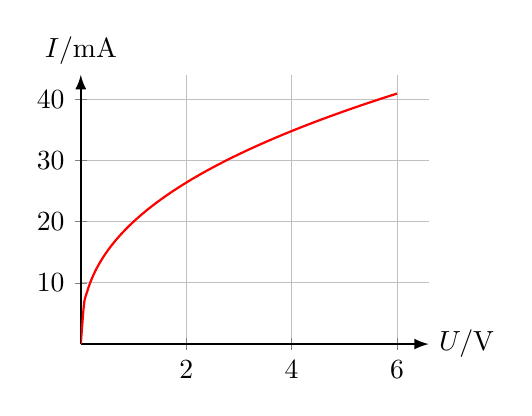
\begin{tikzpicture}
\begin{axis}[
  width=6cm,
  height=5cm,
  domain=0:6,
  samples=100,
  axis y line=middle,
  axis x line=middle,
  xlabel={$U/\si{\V}$},
  ylabel={$I/\si{\milli\A}$},
  xlabel style={right},
  ylabel style={above},
  xmin=0, xmax=6.6,
  ymin=0, ymax=44,
  grid,
  thick,
  smooth
  ]
  \addplot[red] { 20*x^(2/5) };
\end{axis}
\end{tikzpicture}
\end{document}
